\chapter{Machine Learning and uncertainty quantification}
\label{methods_ML}

\vspace{-45pt} % one line spacing corresponds approx to 15 pts
\begin{tcolorbox}[enhanced,width=\textwidth,size=fbox,
        sharp corners,colframe=black!5!white,drop fuzzy shadow southeast,
        boxrule=3mm, parbox=false] 
        
This chapter borrows from the article \citep{walch_big_2020}:

\qquad \bibentry{walch_big_2020}

and the conference proceedings \cite{walch_spatio-temporal_2019, walch_fast_2019-1}:

\quad \bibentry{walch_spatio-temporal_2019} 

\quad \bibentry{walch_fast_2019-1}
\end{tcolorbox}

The large-scale estimation of HyREP at high spatial and temporal resolution challenges analytical and geospatial models as described above, for three main reasons.
First, some data required to perform the analytical and geospatial modelling may not be available across the entire region for which the HyREP is computed.
Second, the resolution or quality of some of the input datasets may be insufficient to assure a high-resolution potential estimation, but it could be improved through the use of additional information.
Third, these physics-based approaches may be too computationally intensive, inhibiting their application at the large scale.
The use of Machine Learning (ML) as a method to address the above limitations of "classical" physics-based models has attracted increasing attention in recent years \cite{willard_integrating_2020}. 

In this thesis, we use ML to address several of the above-mentioned limitations for the national-scale estimation of RPV (Chapter~\ref{solar}) and GSHP (Chaper~\ref{geothermal}) potential. 
To this aim, ML is used in two contexts: 
(i) To learn and predict the relationship between a set of input data (\textit{features}) and output variables (\textit{targets}), known as \textit{supervised learning}, 
and (ii) to group data based on similarities in its features and to identify outliers, known as \textit{clustering}. 
\nomenclature[A]{ML}{Machine Learning}

The use of data-driven methods further requires the estimation of uncertainties related to the ML predictions, which are essential if the outputs are used in decision-making processes \cite{knusel_argument-based_2020}. 
Uncertainties may arise for example from input data sources or from modelling approaches themselves, and their quantification itself is a vast field of research \cite{willard_integrating_2020,knusel_argument-based_2020}.
We use an approach for modelling uncertainty arising from data noise and from the ML model in the form of standard deviations, which we propagate through the analytical models presented in Chapter~\ref{methods_physical}. 
The following sections will provide an overview of the supervised learning and clustering algorithms used in this thesis, as well as the applied methods for a systematic quantification of uncertainties through combined physics-based and data-driven modelling approaches.

\section{Supervised learning algorithms}
\label{ML_supervised}
% Often regarded as black-box models, ML algorithms are trained based on a set of input data (called features), such as to predict an output (the target or label). 
The architecture of each model is determined through a tuning procedure in the training phase, where the parameters defining the model structure (hyper-parameters) are optimized in order to minimize the difference between the prediction and the target. 

\subsection{Feature analysis and selection techniques}


\subsection{Regression models}
\label{ML_models}
\label{RF}
Throughout this work, we use and compare the performance of six supervised regression models from different families of ML algorithms: (i) Linear Regression (LIN), (ii) K-Nearest Neighbors (KNN), (iii) Support Vector Machines (SVM), (iv) Random Forests (RF), Artificial Neural Networks (ANN), and (iv) Extreme Learning Machine Ensembles (ELM-E).
\nomenclature[A]{LIN}{Linear Regression}
\nomenclature[A]{KNN}{K-Nearest Neighbours}
\nomenclature[A]{SVM}{Support Vector Machine}
\nomenclature[A]{RF}{Random Forest}
\nomenclature[A]{ANN}{Artificial Neural Network}
\nomenclature[A]{ELM}{Extreme Learning Machine}
\nomenclature[A]{ELM-E}{ELM Ensemble}
The ML algorithms and their hyper-parameters are summarized below and shown in Fig. 3. 
We use the ML implementations of the \textit{Scikit-learn} library for python \cite{pedregosa_scikit-learn:_2011} for all models except the ELM-E. As no functional open-source code for the ELM-E was available when this work was carried out, we have implemented the ELM-E ourselves using the ELM model of the \textit{HPELM} package for python \cite{akusok_high-performance_2015}, which supports computational acceleration on graphical processing units (GPUs).
\nomenclature[A]{GPU}{Graphical Processing Units}


\begin{figure}[tb] % !
\centering
\makebox[\linewidth][c]{
\begin{subfigure}[t]{.3\textwidth}
  \centering
  \fbox{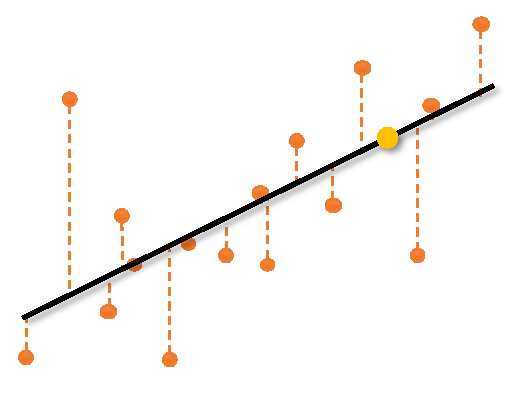
\includegraphics[width=.9\linewidth]{images/Figs/lin.pdf} } 
  \subcaption{\textbf{LIN}}
  \label{fig:lin}
\end{subfigure}
\begin{subfigure}[t]{.35\textwidth}
  \centering
  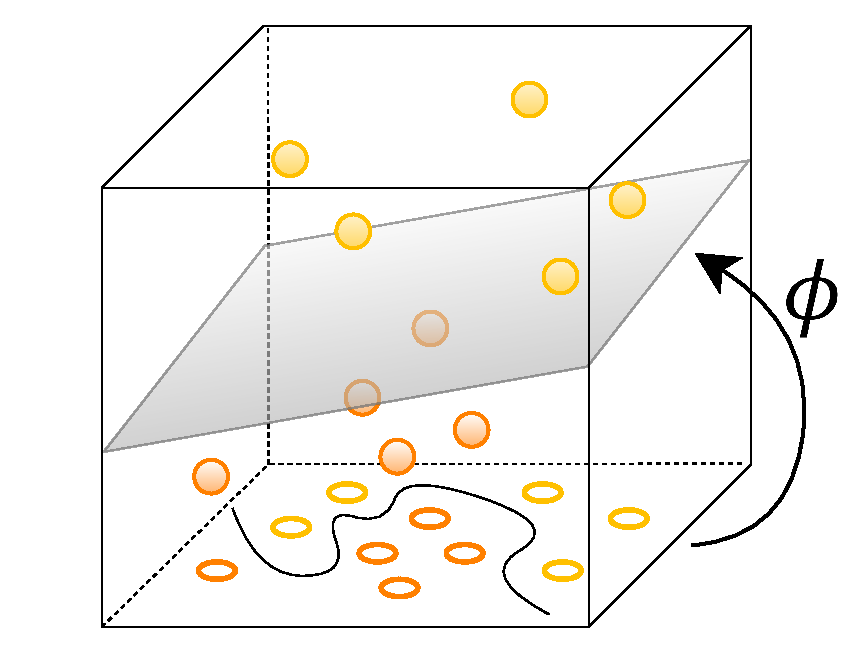
\includegraphics[width=.9\linewidth]{images/Figs/SVM.pdf} 
  \subcaption{\textbf{SVM}}
  \label{fig:svm}
\end{subfigure}
\begin{subfigure}[t]{.35\textwidth}
  \centering
  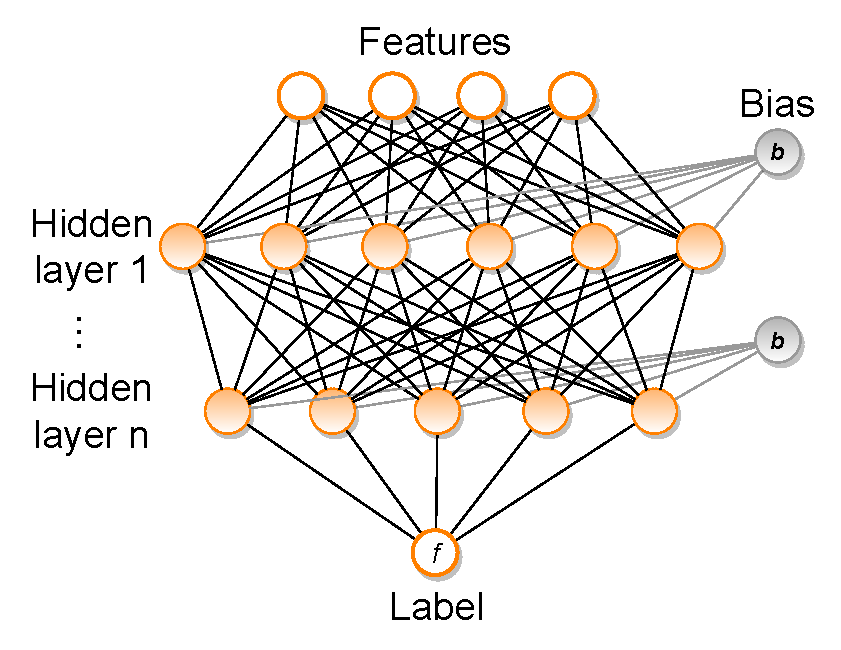
\includegraphics[width=.95\linewidth]{images/Figs/ANN.pdf}
  \subcaption{\textbf{ANN}}
  \label{fig:ann}
\end{subfigure}
} \\ \vspace{.25cm}
\makebox[\linewidth][c]{
\begin{subfigure}[t]{.3\textwidth}
  \centering
  \fbox{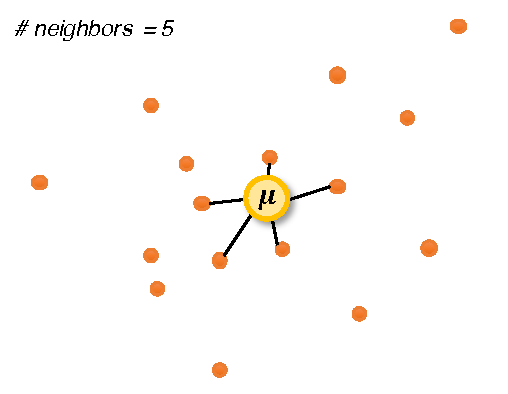
\includegraphics[width=.9\linewidth]{images/Figs/knn.pdf} }
  \subcaption{\textbf{KNN}}
  \label{fig:knn}
\end{subfigure}
\begin{subfigure}[t]{.35\textwidth}
  \centering
  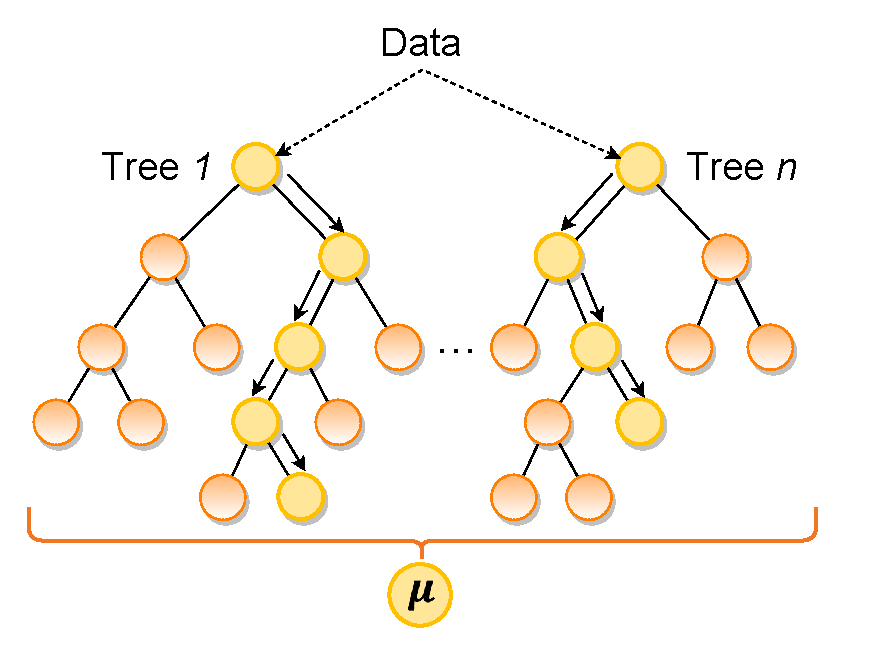
\includegraphics[width=.95\linewidth]{images/Figs/RF.pdf}
  \subcaption{\textbf{RF}}
  \label{fig:rf}
\end{subfigure}
\begin{subfigure}[t]{.35\textwidth}
  \centering
  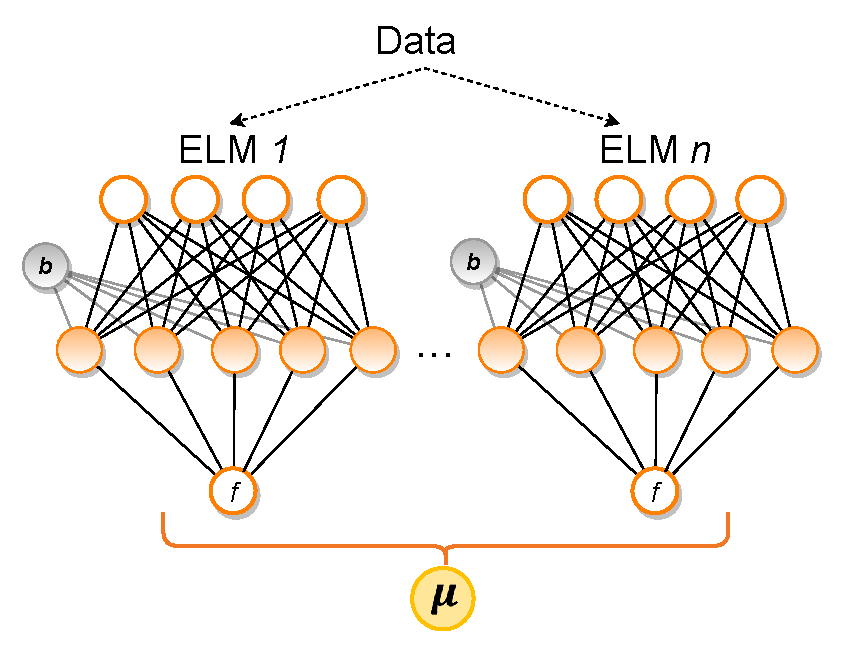
\includegraphics[width=.95\linewidth]{images/Figs/ELM_E.pdf}
  \subcaption{\textbf{ELM-E}}
  \label{fig:elme}
\end{subfigure}
}
\caption{Visualisation of ML algorithms used in this work. The selected algorithms are (a) Linear regression (LIN), (b) K-Nearest Neighbor Regression (KNN), (c) Support Vector Machine (SVM), (d) Random Forest (RF), (e) Artificial Neural Network (ANN), (f) Extreme Learning Machine Ensemble (ELM-E).}
\label{fig:ml_algorithms}
\end{figure}

\textbf{Linear Regression }assumes that the target is a linear function of the inputs. The prediction is obtained from the linear combination of the features which minimizes the residual sum of squares between the target and predicted values. It is fast and requires no tuning of hyper-parameters but shows a low accuracy for non-linear problems.

\textbf{K-nearest Neighbor Regression} is an interpolation algorithm, which computes a prediction as the average of the targets of the $k$ training samples whose features are closest to the given inputs. The training dataset hence works as a look-up table for the predictions, which makes it effective for low-dimensional problems but inefficient for large datasets. We use the Euclidean distance as a measure of “closeness” and tune the number of neighbors ($k$).

\textbf{Support Vector Machine}, introduced by \citet{cortes_support-vector_1995}, is the most popular algorithm in the family of kernel methods. It exploits the \textit{kernel trick}, which projects the features to a higher-dimensional space that allows for linear modelling. Its structure makes it particularly effective for high-dimensional problems, but it does not scale well with the number of samples. In this work, we use $\varepsilon$-Support Vector Regression with a radial basis function as kernel and tune the kernel coefficient ($\gamma$), the penalty parameter (C) and the error tolerance ($\varepsilon$).

\textbf{Random Forest} is an ensemble (i.e. an aggregation) of decision trees, which was proposed by \citet{breiman_random_2001}. Each of the decision trees in. the ensemble pass a training sample along a set of nodes based on a threshold (defined during training) until a leaf node is reached. The prediction of each tree is obtained by averaging the target values in the respective leaves. It is a popular algorithm due to its good predictive power and high robustness. Its main hyper-parameters are the number of features considered for the optimization of each threshold ($m_{ftrs}$), the minimum number of samples in each leaf ($m_{leaf}$) and the number of trees in the ensemble ($n_{est}$).
% A COMMENT ON FEATURE IMPORTANCE

\textbf{Artificial Neural Networks}

\textbf{Extreme Learning Machine Ensemble } is a collection of single-layer neural networks (ELMs), which were developed by \citet{huang_extreme_2006}. Each ELM consists of one hidden layer, which is optimized in a more efficient way than traditional neural networks (see above). This results in a faster training time and a low number of hyper-parameters. The aggregation of $n$ ELMs in an ensemble further increases the robustness of the model and reduces the risk of overfitting. We tune the size of the hidden layer ($m_{ELM}$) and the number of ELMs in the ensemble ($n_{ELM}$).

% A SUBSECTION ON ENSEMBLES, OR SIMPLY TWO PARAGRAPHS

\begin{comment}
% SOURCE: ICAE conference paper
Extreme Learning Machines, as proposed by Huang et al. [11], are single-layer feed-forward neural networks which are trained using a single-step optimization. The training process of ELM is up to hundreds of times faster than the training of other machine learning algorithms [11]. For our model we aggregate M ELM to an ensemble, as shown in Fig. 1. This is known to improve the generalization performance by reducing the risk of overfitting [6,9,12], and allows to estimate the uncertainty as described in Section 2.2. At the hidden layer of each ELM, the training points $x_i$ of dimensionality d are multiplied by the randomly chosen input weights w and added to the random bias b. An activation function ƒ( ) is applied to the resulting random projections for modelling nonlinear behaviour of the data. We use a sigmoid activation function in this study, which is a common choice for regression problems [12]. The hidden layer is multiplied by the output weights $\beta$ and summed to give the model output $\hat{y}i$ (see Eq.1). During training, only $\beta$ needs to be optimized.

For ensemble training, we apply a bootstrap-aggregating (bagging) approach [13] where each ensemble member is trained on one bootstrapped resample of the training data. Each bootstrap replicate is obtained by resampling the N training samples N times uniformly and with replacement. On average, every replicate contains 63.2\% of the original data, with some duplicated samples. At the output, the predictions $\hat{y}_\mathrm{i}^\mathrm{m}$ of each ELM are averaged to give the final estimation $\hat{y}_i$ as shown in Eq. 2. The generation of M bootstrap replicates comes at a computational cost. For the implementation of each ELM, we therefore use the python toolbox hpelm with GPU acceleration [14]. This showed significant speed-up in performance compared to the standard CPU implementation. This implementation allows us to train and to test ELM ensembles with a large number of hidden neurons on our large environmental dataset.
% EQUATIONS 1 and 2 IN ICAE PAPER

\end{comment}



\subsection{Classification models}

 
\section{Clustering techniques}
\subsection{K-means clustering}
\subsection{Density-Based Spatial Clustering of Applications with Noise}


\section{Uncertainties}
\subsection{Uncertainty estimation for ensemble models}
\label{unc_ML}

% SOURCE: Initial submission PV paper
The ensemble structure of both ML algorithms used in this work permits the estimation of uncertainties arising from the modelling process (model uncertainty, $\Hat{\sigma_M}$). The remaining residuals after the subtraction of the model variance are further used to estimate the uncertainty related to the data noise (data uncertainty, $\Hat{\sigma_D}$). 
This approach enables a specific characterization of the uncertainty for each spatio-temporal point.
It has been previously used to estimate, for example, wind speed or global solar radiation~\cite{walch_spatio-temporal_2019, wan_probabilistic_2014}.

The ensemble method is based on a bagging (bootstrap-aggregating) approach, which introduces randomness into the model  \cite{breiman_bagging_1996}.
Every ensemble member is trained on one bootstrapped resample of the training data, which is
obtained by sampling the training set uniformly and with replacement.
The model uncertainty is quantified as the standard deviation of the predictions of all model in the ensemble, which is computed as:

\begin{equation}
\label{eq:model_unc}
  \Hat{\sigma}_M^2 (\mathbf{x}_i) = \frac{1}{N} \sum_{n=1}^N (\Hat{y}_i^n - \Hat{y}_i)^2, \quad i=1,...,L
\end{equation}

where $\Hat{\sigma}_M$ denotes the model standard deviation, referred to as model uncertainty, $N$ denotes the ensemble length, $\Hat{y}_i$ is the ensemble prediction for sample $\mathbf{x}_i$ and $\Hat{y}_i^n$ is the prediction of ensemble member $n$.

Additionally to the model variance, we estimate the variance of the data noise by modelling the remaining residuals. They are derived by subtracting the model variance from the squared difference between $\Hat{y}_i$ and the targets $t_i$, as shown below.
In order to reduce bias, the out-of-bag (OOB) model output are used, which is the mean of the ensemble members for which a given training data point was not considered (due to bootstrapping) \cite{heskes_practical_1997}. 

\begin{equation}
\label{eq:data_unc}
  \Hat{\sigma}_D^2 (\mathbf{x}_i) = \max \{ (t_i - \Hat{y}_i)^2 - \Hat{\sigma}_M^2 (\mathbf{x}_i) , 0 \}, \quad i=1,...,L
\end{equation}
 
 where $\Hat{\sigma}_D$ denotes the standard deviation of data noise, referred to as data uncertainty, and $t_i$ is the target value for sample $\mathbf{x}_i$. 
$\Hat{\sigma}_D$ can only be computed if $t_i$ is known. Thus, a second ML model is trained from the residuals to predict $\Hat{\sigma}_D$ for points with unknown targets. Unless mentioned otherwise, the same hyper-parameters are used in both models.

The total variance of a variable that is estimated using a ML model is the squared sum of its model uncertainty and its data uncertainty: 

\begin{equation}
\label{eq:total_unc}
\sigma^2 (\mathbf{x}_i) = \Hat{\sigma}_M^2 (\mathbf{x}_i) + \Hat{\sigma}_D^2 (\mathbf{x}_i), \quad i=1,...,L
\end{equation}

% Source: ICAE paper
% Applying bagging to the ELM ensemble increases the quality of the prediction and it also allows to compute the model uncertainty $\hat{\sigma}M$, derived from the variance ${\hat{\sigma}}_M^2$ of the M model outputs ${\hat{y}}_\mathrm{i}^\mathrm{m}$ (see Eq. 3) [9,15]. Afterwards, remaining residuals are derived by subtracting the model variance from the squared difference between the model outputs and the targets ti, as visible in Eq. 4. We compute these residuals for the training data, which are used to train a second ELM ensemble. The output is the data noise variance ${\hat{\sigma}}_D^2$, and the standard deviation $\hat{\sigma}D$ quantifies the data uncertainty. Adding model and data noise variance provides a qualitative estimate of the uncertainty on the predictions.

\begin{comment}
\subsubsection{Uncertainty for GIS methods}

The uncertainty for the GIS-derived and bias corrected quantities, namely $S_{sh}$ and $SVF$, is estimated from the residuals between the values computed using the $(2 \times 2)m^2$ and the $(0.5 \times 0.5)m^2$ resolution DSM in Geneva. The latter is considered the "true" surface model. 
The error in the GIS-derived quantities is treated as a random variable, whose first and second moments are estimated from the mean and the variance of the discrepancy. The mean is used for the bias correction, as explained in Sections \ref{shade} and \ref{svf}, while the variance represents the uncertainty.

It should be noted that the error of the GIS methods for $C_{sh}$ and $C_{pv}$ are not computed in the way described here, as they form part of the data uncertainty estimated by the subsequent ML models.
\end{comment}

\subsection{Uncertainty propagation}
\label{method_unc_prop}

% SOURCE: Initial submission PV paper
The correlation among the random variables plays a key role in the propagation of uncertainty. If statistical independence can be assumed, the mean and variance of the resulting variables can be computed from the mean and variance of each parameter only, which greatly simplifies the uncertainty propagation.
% As the uncertainty is computed separately for each spatio-temporal data point, we assume statistical independence between meteorological and building related parameters, namely between $G_h, G_B, G_D$ and $S_{sh}, SVF, A_{PV}$. This is valid as the uncertainty of the horizontal radiation is dominated by the meteorological conditions, while those of $S_{sh}(t), SVF, A_{PV}$ are related to the GIS and ML methods. These are independent and uncorrelated processes.

In error propagation theory~\cite{jcgm_evaluation_2008, goodman_variance_1962}, the uncertainty on the final measurand is the result of the propagation over a set of sums and products of its variables. In error analysis, the variance of the sum of $N$ randomly distributed variables $X_i$ is given by:

\begin{equation}
\label{eq:unc_sum}
\mathrm{Var}\left(\sum_{i=1}^N X_i\right) = \sum_{i=1}^N\mathrm{Var}(X_i) + 2\sum_{i < j}\mathrm{Cov}(X_i, X_j)
\end{equation}

Following the considerations and approximations detailed above, we can further regard all multiplications of the variables forming the measurand as statistically independent. 
The variance of the product of two independent randomly distributed variables $X$ and $Y$ is given by:

\begin{equation}
\label{eq:unc_prod}
\mathrm{Var}(XY) = \mathrm{Var}(X)\mathrm{Var}(Y) + \mathrm{Var}(X) \mathrm{E}(Y)^2 + \mathrm{Var}(Y) \mathrm{E}(X)^2
\end{equation}
%% ADD FULL EQUATION WITH COVARIANCES

%\section{Optimisation of hybrid energy systems}
